\documentclass[10pt,a4paper]{article}
\usepackage[margin=2.2cm]{geometry}
\usepackage{fontspec}
\usepackage{xeCJK}
\setCJKmainfont{SimSun}[BoldFont=SimHei]
\setCJKsansfont{SimHei}
\usepackage{amsmath}
\usepackage{graphicx}
\usepackage{booktabs}
\usepackage{array}
\usepackage{caption}
\usepackage{enumitem}
\usepackage{float}
\usepackage[hidelinks]{hyperref}
\setlist{nosep,leftmargin=1.5em}
\setlength{\tabcolsep}{4pt}
\linespread{1.22}
\captionsetup{font=small}
\renewcommand{\figurename}{图}
\renewcommand{\tablename}{表}
\newcolumntype{L}[1]{>{\raggedright\arraybackslash}p{#1}}
\newcommand{\dn}{\Delta n_0}

\title{\textbf{长孔径分段馈电薄膜铌酸锂声光相位调制器：\\数据汇总与后续工作}}
\author{陈鑫磊\quad 上海电力大学}
\date{2026 年 10 月 23 日}

\begin{document}
\maketitle

\noindent\fbox{\parbox{\dimexpr\linewidth-2\fboxsep-2\fboxrule}{\small
\textbf{本稿仅限课题组内部：仿真与方案工作稿，实测待做，无伪造数据，Fiber-Q 未下单，无流片；不得作为公开或可引用结果。}
文中全部器件数字均为 COMSOL 仿真预测或由仿真数据换算，不是实验结果；标明“假设”“建议”“估计”的数字不是计算或测量所得。}}

\section{现状概览}
仿真层面的链路已经走通：二维截面（取向、脊高、光弹与电光耦合）$\rightarrow$ 三维分段单元（汇流条、指端、段间隙）$\rightarrow$
支撑梁 $\rightarrow$ 两侧引线与馈电网络 $\rightarrow$ 空气桥光吸收。各环节在模型范围内\textbf{没有发现阻断性问题}，
$L = 1$ mm 的信号源功率在计入各项后约为 3.3 mW（仿真）。但这不等于设计已验证：绝对数值有数倍不确定度，
光学过渡、沿波导方向的声学端部、机械强度等尚未覆盖（见第~\ref{sec:cov} 节）。

\begin{table}[H]
\centering\small
\caption{头条数据（仿真预测；$L = 1$ mm，2 串 $\times$ 5 并，$50\ \Omega$ 信号源）}\label{tab:head}
\begin{tabular}{L{4.4cm}L{3.3cm}L{7.6cm}}
\toprule
项目 & 数值 & 条件与来源 \\
\midrule
谐振频率 & 3.333 GHz & 三维，周期 1.84 µm；二维有限长低约 5 MHz \\
驱动 $Q$ & 1930--1970 & 由假设的损耗因子 $\eta_s = 5\times10^{-4}$ 给出，\textbf{非测得} \\
单位长度效率 $P_\pi L$ & $2.58\times10^{-6}$ W·m & 100 µm 段、汇流条 0.5 µm，为无汇流条的 1.10 倍；加支撑梁 $2.87\times10^{-6}$ \\
所需信号源功率 $P_\pi$ & \textbf{3.26 mW} & 含支撑梁、梁上走线、500 nm 铝引线与焊盘；薄铝窄轨最差约 3.7 mW \\
同上，经模型校准 & 5.5--17 mW & 乘校准系数 1.7--5.3（二维流程对 Shao 结构 $\dn$ 偏高 1.3--2.3 倍） \\
等效电压（匹配负载端峰值） & 0.57 V（校准后 0.74--1.3 V） & $V=\sqrt{2R_0P}$；定义与匹配条件和文献 $V_\pi$ 不同，不能直接比较 \\
输入阻抗 & 53--57 $\Omega$ & 节点网络，含引线轨 \\
段间失谐影响 & $\sigma = 1$ MHz 时 $\times1.27$ & 2 串 $\times$ 5 并中位数；全并联 $\times1.08$ \\
空气桥光吸收 & 可忽略 & 桥底离脊顶 0.5 µm 时每座约 $4\times10^{-5}$ dB \\
$L = 2$ mm（粗估） & 约 1.8 mW & 未计梁和引线时为 1.55 mW，按 1 mm 的 $\times1.14$ 外推，未单独计算 \\
\bottomrule
\end{tabular}
\end{table}

与 Shao 等（Optica 2019）同一流程、同段长比较，本设计的单位长度效率为 Shao 型的 0.77--0.87 倍，
即\textbf{单位长度效率没有明显超过 Shao 型}；可主张的差别在于毫米级孔径加分段串并联后能配到 $50\ \Omega$。

\section{当前设计}
\begin{table}[H]
\centering\small
\caption{设计参数（仿真所用值）}
\begin{tabular}{L{3.0cm}L{12.4cm}}
\toprule
类别 & 参数 \\
\midrule
材料与取向 & 悬空 X 切铌酸锂，平板 400 nm，脊高 400 nm；Shao 取向（声沿晶体 Z，TE 光沿晶体 Y，主要利用 $r_{33}$ 与光弹效应）；波长 1550 nm \\
叉指 & 周期 1.84 µm，铝，指宽 $0.25p$，厚 100 nm；波导嵌在叉指中间（NP = 7，中间 3 个周期放波导） \\
分段 & $L = 1$ mm = 10 段 $\times$ 100 µm；段间隙 0.5 µm，汇流条 0.5 µm，指端间隙 0.5 µm \\
支撑梁 & 每个段间隙两侧各一根，宽 2 µm、长 6 µm（仿真取远端 4 µm PML），梁上 100 nm 铝走线引出信号与地 \\
接法 & 2 串 $\times$ 5 并，相邻串镜像排列，段间隙电位依次为信号 / 浮空 / 地 / 浮空；浮空间隙不需引出 \\
引线 & 锚区引线轨，两侧各一对信号与地（A 型）；500 nm 铝，信号轨 50 µm、间隙 10 µm、地轨 100 µm（假设） \\
衬底（假设） & 锚区叠层 LN 400 nm / SiO$_2$ 2 µm / 高阻 Si 500 µm，按无损介质处理 \\
\bottomrule
\end{tabular}
\end{table}

\section{数据汇总}
\subsection{功率如何一步步演变}
图~\ref{fig:chain}(a) 给出 $L = 1$ mm 所需功率随模型逐步完善的变化：三维汇流条与指端使功率从二维的 2.46 mW 升到 3.90 mW，
汇流条减窄和周期回调后降到 2.85 mW，支撑梁（$\times1.11$）与真实引线（$+3$--$4\%$）使其回升到 3.26 mW，约为二维结果的 1.3 倍。
图~\ref{fig:chain}(b) 是段间失谐的影响，见第~\ref{sec:tol} 节。

\begin{figure}[H]
\centering
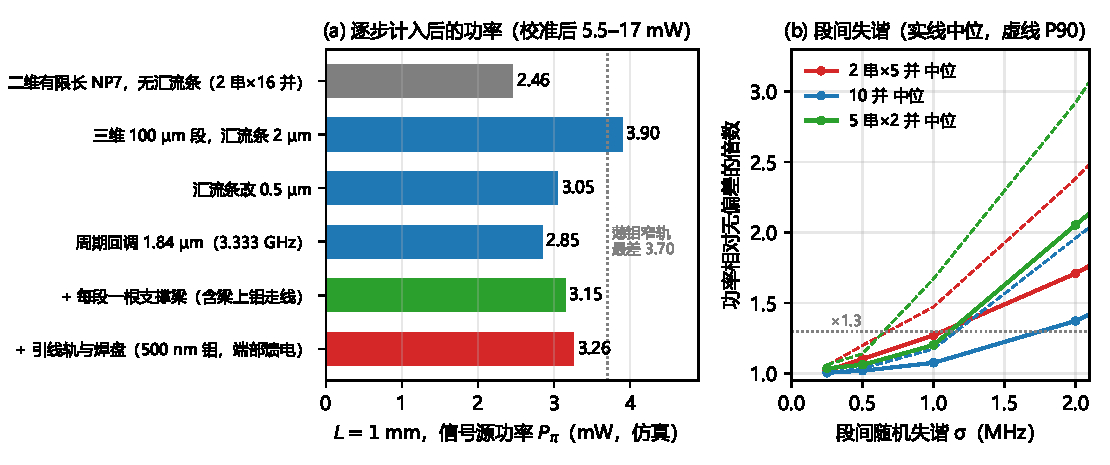
\includegraphics[width=0.98\linewidth]{fig_chain.pdf}
\caption{(a) $L = 1$ mm 信号源功率（仿真）。第一条为二维有限长（2 串 $\times$ 16 并）；第 2--4 条为三维 100 µm 段、2 串 $\times$ 5 并，未计梁和引线；第 5、6 条逐项计入梁与引线。
(b) 段间随机失谐对功率的影响（周期 1.84 µm，$L = 1$ mm，每点 100 次随机）。}\label{fig:chain}
\end{figure}

\subsection{单位长度效率：段长、汇流条与周期}
\begin{table}[H]
\centering\footnotesize
\caption{三维结果（$P_\pi L$ 单位 $10^{-6}$ W·m；网格为截面 250 nm、沿波导 1--1.5 µm；25 µm 段对沿波导网格敏感，只给区间）}\label{tab:pl}
\begin{tabular}{L{5.4cm}cccc}
\toprule
配置 & $f$ (GHz) & $P_\pi L$ 主峰 & 相对无汇流条 & 周期 (µm) \\
\midrule
二维有限长 FN7 & 3.211 & 2.43 & --- & 1.9277 \\
三维无汇流条 & 3.216 & 2.49 & 1 & 1.9277 \\
25 µm 段，汇流条 2 µm & 3.21 & 4.8--8.6 & 1.9--3.4 & 1.9277 \\
50 µm 段，汇流条 2 µm & 3.217 & 5.09 & 2.0 & 1.9277 \\
100 µm 段，汇流条 2 / 1 / 0.5 µm & 3.217 / 3.217 / 3.216 & 3.58 / 3.76 / 2.76 & 1.44 / 1.51 / 1.11 & 1.9277 \\
\midrule
三维无汇流条 & 3.333 & 2.34 & 1 & 1.84 \\
\textbf{100 µm 段，汇流条 0.5 µm} & \textbf{3.333} & \textbf{2.58} & \textbf{1.10} & 1.84 \\
再加支撑梁与梁上走线 & 3.333 & 2.87 & 1.22（相对无梁 1.11） & 1.84 \\
\midrule
Shao 型（同流程，直壁近似），25 / 100 µm 段 & 3.19 & 8.4 / 4.1 & 2.5 / 1.23 & --- \\
\bottomrule
\end{tabular}
\end{table}

\begin{itemize}
  \item 汇流条与指端使主模分裂成一串间距 0.3--1 MHz 的模式，损失随段长减小；100 µm 段只剩一个干净主峰。这一损失不是本设计特有，同流程下 Shao 型同样出现。
  \item 汇流条宽度：周期 1.9277 µm 时 1 µm 处有一个旁模并入主峰（无收益）；周期 1.84 µm 下细扫 0.3 / 0.4 / 0.5 / 0.6 / 0.7 µm，
        $P_\pi L$ 为 2.53 / 2.56 / 2.58 / 2.72 / 2.79，单调平滑、无旁模，$L = 1$ mm 为 2.81 / 2.84 / 2.85 / 3.01 / 3.06 mW。
  \item 周期回调：二维 $f$ 对周期斜率约 $-1.33$ MHz/nm，由 1.9277 µm 回调到 1.84 µm 把主峰移到 3.333 GHz，$P_\pi L$ 同时降约 7\%。
\end{itemize}

\begin{figure}[H]
\centering
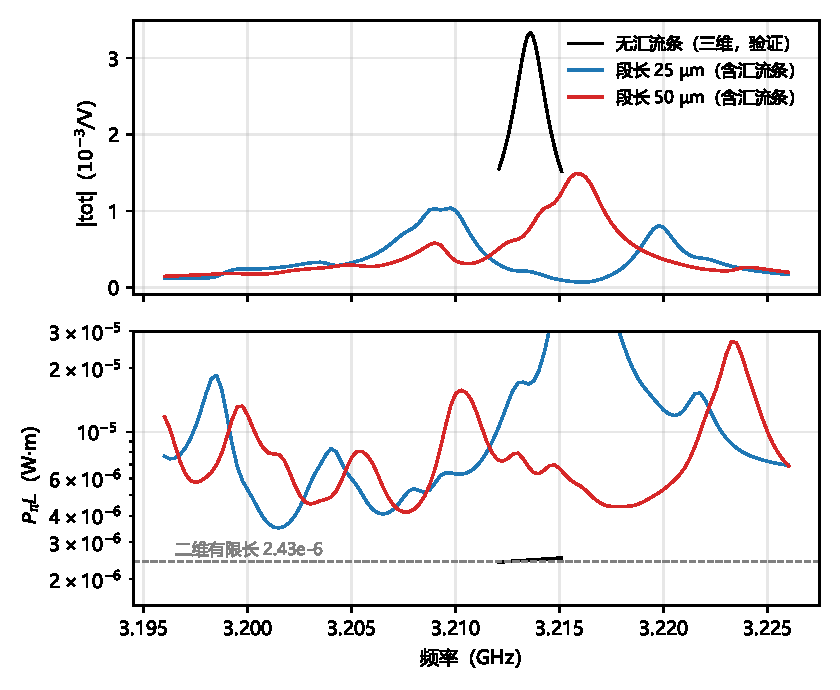
\includegraphics[width=0.92\linewidth]{fig_3d.pdf}
\caption{三维分段单元的频域驱动响应（周期 1.9277 µm，汇流条 2 µm）。(a) 本设计不同段长的调制系数 $|{\rm tot}|$；(b) 主峰 $P_\pi L$ 随段长的变化，点线为各自无汇流条的值。}
\end{figure}

\subsection{工艺容差与段间失谐}\label{sec:tol}
\begin{table}[H]
\centering\small
\caption{工艺偏差对单段的影响（二维有限长，周期 1.9277 µm，基准 3.2113 GHz、$2.434\times10^{-6}$）}
\begin{tabular}{L{6.0cm}ccc}
\toprule
偏差 & $\Delta f$ & $P_\pi L$ 变化 & 备注 \\
\midrule
膜厚 $-10$ / $+10$ nm（脊 400 nm 不变） & $+4.2$ / $-4.4$ MHz & $+0.3\%$ / $-0.2\%$ & $-0.43$ MHz/nm \\
刻蚀浅 / 深 10 nm（总厚不变） & $-0.1$ / $0$ MHz & $+6.9\%$ / $-6.3\%$ & 只影响效率 \\
周期 $\pm1\%$（$\pm$19 nm） & $\mp25$ MHz & 约 $\pm2\%$ & $-1.33$ MHz/nm \\
\bottomrule
\end{tabular}
\end{table}

主峰 FWHM 约 1.7 MHz，段间 1 MHz 的失谐对应约 2.3 nm 膜厚差或 0.75 nm 周期差（周期由光刻一次定义，段间差应远小于 1 nm）。
下表为每段单独加频偏后的馈电网络结果（$L = 1$ mm，每种 100 次随机；基准功率 2 串 $\times$ 5 并 2.89 mW，全并联 3.45 mW，5 串 $\times$ 2 并 5.65 mW）：

\begin{table}[H]
\centering\small
\caption{段间失谐下的功率倍数（中位 / 90\% 分位）}
\begin{tabular}{L{3.2cm}cccc}
\toprule
接法 & $\sigma = 0.5$ MHz & $\sigma = 1$ MHz & $\sigma = 2$ MHz & 线性梯度（两端差 2 MHz） \\
\midrule
2 串 $\times$ 5 并 & 1.10 / 1.20 & 1.27 / 1.47 & 1.71 / 2.38 & 1.31 \\
10 并 & 1.02 / 1.04 & 1.08 / 1.17 & 1.37 / 1.96 & 1.04 \\
5 串 $\times$ 2 并 & 1.06 / 1.14 & 1.20 / 1.67 & 2.05 / 2.92 & 1.63 \\
\bottomrule
\end{tabular}
\end{table}

串联段电流相同、电压按各自阻抗分配，失谐段分到的电压不对；并联段电压相同，能自动均衡。串联越多，最坏情况和线性梯度下越敏感。
功率增量要控制在约 30\% 以内，需 $\sigma$ 在 1 MHz 左右以内，即段间膜厚差约 2.3 nm 以内（$\sigma = 2$ MHz 约 4.7 nm）。
失谐未知时用全并联更稳，基准功率高约 20\%；分界点约在 $\sigma = 1$ MHz。

\subsection{支撑梁、引线与空气桥}
\begin{table}[H]
\centering\footnotesize
\caption{支撑梁（每段间隙一根，上界；100 µm 段，汇流条 0.5 µm，周期 1.84 µm）}
\begin{tabular}{L{3.4cm}cccc}
\toprule
算例 & 驱动 $Q$ & $P_\pi L$ ($10^{-6}$) & 相对无梁 & 1 mm（2 串 $\times$ 5 并） \\
\midrule
无梁 & 1931 & 2.578 & 1 & 2.85 mW \\
梁宽 1 / 2 / 4 µm，PML & 1928 / 1945 / 1960 & 2.860 / 2.850 / 2.856 & 1.109 / 1.105 / 1.108 & 3.13 / 3.13 / 3.15 mW \\
2 µm，远端固定 & 1969 & 2.858 & 1.109 & 3.15 mW \\
2 µm，PML，梁上铝走线 & 1943 & 2.865 & 1.111 & 3.15 mW \\
\bottomrule
\end{tabular}
\end{table}

梁使 $P_\pi L$ 增加约 11\%，几乎不随梁宽和远端条件变化，$Q$ 不降、无新旁模；PML 与固定端相差小于 1\%，
说明锚点漏能可忽略；几何保留但不参与物理场的对照与无梁逐位相同，排除了网格影响。

\begin{table}[H]
\centering\footnotesize
\caption{$L = 1$ mm 所需信号源功率（mW）：引线与接法（假设衬底与金属厚度）}
\begin{tabular}{L{4.8cm}cccc}
\toprule
引线 & 接法 & 馈电位置 & 2 串 $\times$ 5 并 & 全并联 \\
\midrule
理想（各驱动间隙直接接源） & --- & --- & 3.15 & 3.68 \\
500 nm 铝，50 / 10 / 100 µm 轨 & A（两侧走轨） & 端部 / 中点 & \textbf{3.26} / 3.25 & 3.49 / 3.46 \\
 & C（一侧 + 空气桥） & 端部 / 中点 & 3.29 / 3.27 & 3.68 / 3.61 \\
100 nm 铝，20 / 5 / 50 µm 轨（最差） & A & 端部 / 中点 & 3.46 / 3.32 & 3.71 / 3.54 \\
 & C & 端部 / 中点 & 3.70 / 3.42 & 4.13 / 3.75 \\
\bottomrule
\end{tabular}
\end{table}

引线轨（二维静电，各种宽度间隙下）约 0.09--0.13 pF/mm、0.49--0.64 nH/mm、特征阻抗 62--84 $\Omega$；真正有影响的是串联电阻
（100 nm 铝、20 µm 轨为 14 $\Omega$/mm）。厚引线（500 nm、$\ge$ 50 µm）只增加 3--4\%，薄窄轨增加 10--17\%。
空气桥：桥底离脊顶 0.5 µm 时桥下段损耗 0.219 dB/cm（无桥 0.00053 dB/cm），每座（沿波导宽 2 µm）约 $4.4\times10^{-5}$ dB，
1 mm 器件 6 座合计约 $3\times10^{-4}$ dB；$\ge$ 1 µm 时与无桥相同。

\section{覆盖范围与可信度}\label{sec:cov}
\begin{table}[H]
\centering\footnotesize
\caption{已做、假设与未覆盖项}
\begin{tabular}{L{2.3cm}L{4.3cm}L{4.2cm}L{4.0cm}}
\toprule
项目 & 现状 & 可能影响 & 处理 \\
\midrule
绝对数值 & 校准系数 1.7--5.3；$Q\approx2000$ 为假设（Shao 实测 $Q$ 最高约 3600），功率 $\propto 1/Q$ & 功率可能偏差数倍 & 流片后测 $Q$ 与 $P_\pi$，更新校准 \\
光学过渡（悬空与非悬空） & \textbf{未算} & 影响插损和反射纹波，不影响 $P_\pi L$ & 二维模式重叠估计（A1） \\
光纤端面耦合 & \textbf{未算}，与悬空段设计无关 & 只影响总插损 & 沿用成熟耦合结构 \\
沿波导方向的声学端部 & \textbf{未算}：三维取 $z$ 向周期边界，有限长只做了横向 & 端部段响应、侧模、实际 $Q$ & 有限长三维（A2）；长度系列实测 \\
机械强度与应力 & \textbf{未算} & 释放、塌陷、翘曲 & 需工艺侧参数；梁间距变体 \\
衬底、金属厚度、焊盘 & 全部为\textbf{假设值} & 引线损耗与寄生 & 换参数重算只需几分钟（A3） \\
普通阻值硅衬底 & 按高阻无损 & 引线额外损耗 & 实际衬底电阻率重算 \\
探针、键合线、片外功分器 & 未计 & 输入阻抗与带宽 & 测试结构去嵌入 \\
真实侧壁角（斜壁） & 三维未做；Shao 对照用直壁近似 & $\dn$、$f$ 的敏感度未知 & A4 \\
段间膜厚均匀性 & 未假设具体数值 & $\sigma$ 超过 1 MHz 时功率明显上升 & 查晶圆规格；全并联保底 \\
查新 & 只做网页检索（英文 6 次、中文 1 次） & 不能替代正式查新 & 查 WoS、CNKI、专利库全文（A8） \\
\bottomrule
\end{tabular}
\end{table}

\section{后续工作}
\subsection{流片前的仿真与核对}
\begin{table}[H]
\centering\footnotesize
\caption{仿真与核对任务（耗时为估计，判据为建议值）}
\begin{tabular}{L{0.8cm}L{5.6cm}L{2.0cm}L{4.4cm}L{1.2cm}}
\toprule
编号 & 内容与方法 & 估计耗时 & 判据（建议） & 优先级 \\
\midrule
A1 & 光学过渡：分别求悬空与非悬空截面的 TE0，做重叠积分，估计突变过渡的透射与反射，用二维模式求解流程即可，不做三维全波 & 约半小时 & 单个过渡损耗按插损预算定；若到零点几 dB 以上，版图里加锥形过渡 & 高 \\
A2 & 沿波导方向的声学端部：取 3--5 段有限长三维模型，端部分别设 PML、固定、自由，与周期结果比较 $P_\pi L$、$Q$、侧模；\textbf{先估算内存} & 数小时到一天 & 端部段对总响应的影响 $<$ 数十 \%；若内存不足，改迭代求解器、缩小横向域或减段数 & 中 \\
A3 & 换入实际参数：来料膜厚、BOX 厚度、金属厚度、衬底电阻率、焊盘尺寸，重算周期中心值与馈电网络 & 参数到手后 $<$ 1 小时 & 周期中心值按实际膜厚平移：膜厚每偏 1 nm 约需把周期反向调 0.32 nm（0.43 / 1.33，估算） & 高 \\
A4 & 斜壁三维：把界面移动项推广到斜面，评估侧壁角对 $\dn$ 和 $f$ 的影响 & 半天到一天 & 灵敏度小则无需处理 & 低 \\
A5 & 更稀疏的梁：每 2 段（或更多）一根，验证声学损失；先估内存 & 数小时 & 损失 $\le$ 1.3 倍、$Q$ 降 $\le$ 20\%（沿用此前标准） & 中 \\
A6 & 梁长与 PML 长度的敏感度（目前只算 6 + 4 µm 一组） & 1--2 小时 & 结果变化 $<$ 数 \% & 低 \\
A7 & 机械：梁与空气桥的强度、薄膜应力、释放后翘曲 & 取决于工艺参数 & 工艺侧给出应力与释放条件 & 高 \\
A8 & 正式查新：WoS、CNKI、专利库全文 & 外部 & --- & 中 \\
\bottomrule
\end{tabular}
\end{table}

\noindent 建议顺序：先要来实际工艺参数（A3、A7），同时做 A1；之后看内存估算结果再决定 A2、A5；A4、A6 可后置。
下单前建议确认：机械可加工性（工艺侧）、光学过渡无明显问题、版图里带有全并联保底变体。

\subsection{流片版图变体（建议）}
一个设计一个版本的风险太大，建议做成扫描。下表是建议的变体组，具体档位受代工厂设计规则和掩模网格限制，待确认。

\begin{table}[H]
\centering\footnotesize
\caption{版图变体建议}
\begin{tabular}{L{0.8cm}L{4.9cm}L{4.4cm}L{4.5cm}}
\toprule
组 & 变体 & 目的 & 对应仿真预测 \\
\midrule
G1 & 主设计：10 段 $\times$ 100 µm，2 串 $\times$ 5 并，汇流条 0.5 µm，周期 1.84 µm，每段间隙一根 2 µm 梁，500 nm 铝引线 & 基准 & 3.333 GHz；3.26 mW；$Q$ 假设 2000 \\
G2 & 同几何、全并联（10 并） & 失谐未知时的保底 & 3.46--3.68 mW \\
G3 & 周期系列：1.84 µm 为中心，步长约 2 nm，共 5 档（覆盖约 $\pm$5 MHz，相当于膜厚约 $\pm$12 nm） & 测 $f(p)$ 斜率，并让工作点落在目标频率附近；\textbf{若源频率可扫且不要求固定频率，则不是找谐振所必需} & 斜率 $-1.33$ MHz/nm \\
G4 & 长度系列：0.1 / 0.2 / 0.5 / 1 / 2 mm（1 / 2 / 5 / 10 / 20 段） & 测 $P_\pi$ 随长度的变化与端部效应 & 近似 $\propto 1/L$；各点功率需用馈电程序重算 \\
G5 & 段长对照：25 / 50 / 100 µm，同总长 & 验证三维汇流条损失 & 相对无汇流条 3.4 / 2.0 / 1.44（周期 1.9277 µm、汇流条 2 µm 时） \\
G6 & 汇流条宽 0.3 / 0.5 / 0.7 µm（避开 1 µm 附近） & 线宽偏差余量 & $P_\pi L$ 2.53 / 2.58 / 2.79 \\
G7 & 梁变体：宽 1 / 2 / 4 µm；间距每段 / 每 2 段 / 每 5 段 & 机械良率与声学损失的折中 & 每段一根 $\times1.11$；稀疏者未算 \\
G8 & Shao 2019 复刻结构（100 µm） & 在本批工艺上校准方法与系数 & 同流程仿真 $P_\pi L = 2.36\times10^{-6}$（斜壁二维） \\
G9 & 测试结构：无电极悬空波导（光损耗基线，含不同悬空长度以拆出过渡损耗）、单叉指 S11、引线轨 open / short / thru、膜厚与刻蚀深度监测标记、梁与空气桥电阻链 & 把光学、电学参数分开测，便于去嵌入 & 空气桥 $\le 3\times10^{-4}$ dB；引线轨参数见上 \\
\bottomrule
\end{tabular}
\end{table}

\subsection{测量与数据处理}
\begin{itemize}
  \item 电学（VNA）：S11 给出谐振频率、$Q$（FWHM）、Re$Y$ 和输入阻抗，与 3.333 GHz、53--57 $\Omega$ 比较；以长度系列和周期系列检查 $f(p)$ 斜率。
  \item 光学：相位调制边带比或 MZI 偏置法给出 $P_\pi$（或 $V_\pi$）；用 G4 的 $P_\pi$ 对 $L$ 的关系拆出端部效应；用 G9 的光损耗基线扣除过渡与传播损耗。
  \item 校准更新：把实测 $Q$ 代入 $P_\pi L = \hbar\omega^2\lambda^2/(4QL_a\dn^2)$（$L_a = 100$ µm），反推 $\dn$，与仿真比较；
        校准系数 1.7--5.3 是对 Shao 结构得到的，要用 G8 在本批工艺上重新确定。
  \item 以实测的段间谐振分散（G1、G2 的差别）决定最终采用 2 串 $\times$ 5 并还是全并联。
\end{itemize}

\section{风险小结}
\begin{enumerate}
  \item \textbf{模型绝对精度}：校准系数 1.7--5.3、$Q$ 为假设值，功率不确定度数倍。只能靠测试结构或流片确定。
  \item \textbf{机械可行性}：梁与空气桥的强度、应力和释放工艺没有仿真，是目前最需要工艺侧意见的一项。
  \item \textbf{端部与过渡}：光学过渡和沿波导方向的声学端部未建模，影响插损、纹波和端部段响应；A1 成本低，A2 视内存。
  \item \textbf{均匀性}：段间膜厚差要小于约 2.3 nm（$\sigma$ 约 1 MHz 以内）才能保持串联接法的优势；不确定时用全并联。
  \item \textbf{衬底与封装}：高阻 Si、金属厚度、焊盘与探针寄生均为假设或未计。
\end{enumerate}

\section*{附：文件}
\footnotesize\sloppy
仓库 \texttt{dir11/comsol\_ao\_run/step6\_optics/}：二维 \texttt{Step6j.java}、三维 \texttt{Step7.java}、引线 \texttt{Step8Rail.java}、\texttt{Step8Bridge.java}；
后处理 \texttt{post\_step6j\_match.py}、\texttt{post\_step7\_match.py}、\texttt{post\_step7\_spread.py}、\texttt{post\_step7\_beam.py}、\texttt{post\_step8\_feed.py}；
记录 \texttt{summary\_step6i/6j/7/8.md}；本稿作图 \texttt{report/make\_figs7.py}、\texttt{report/make\_figs9.py}。数据均来自上述日志，未做手工修改。

\end{document}
